\section{Extract particles}

 \begin{figure}[H]
  \centering
  \captionsetup{width=.8\linewidth} 
  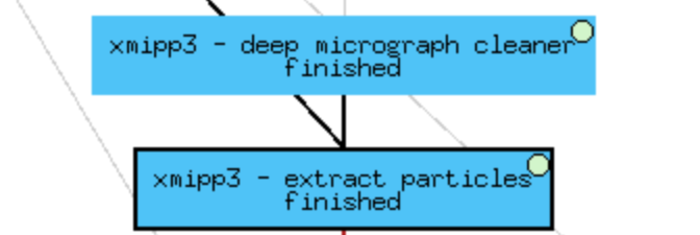
\includegraphics[width=0.35\textwidth]
  {{images/6_workflow4_ExtractParticles.pdf}}
  \caption{Extract particles workflow.}
  \label{fig:workflow_4_a}
  \end{figure}
  
Once we have the set of coordinates, we can proceed to extract particles with \ttt{Xmipp} protocol \scommand{xmipp3-extract particles} (\ffigure{fig:xmipp_extract_particles}). This protocol allows to extract, normalize and correct the CTF phases of the selected particles. As input, this protocol requires the set of coordinates, the consensus CTF values obtained in previous steps, and a downsampling factor. To save computing resources, include in the input the desired reduced size of the particles. In this particular case, 120 pixels.

\begin{figure}[H]
  \centering
  \captionsetup{width=.8\linewidth} 
  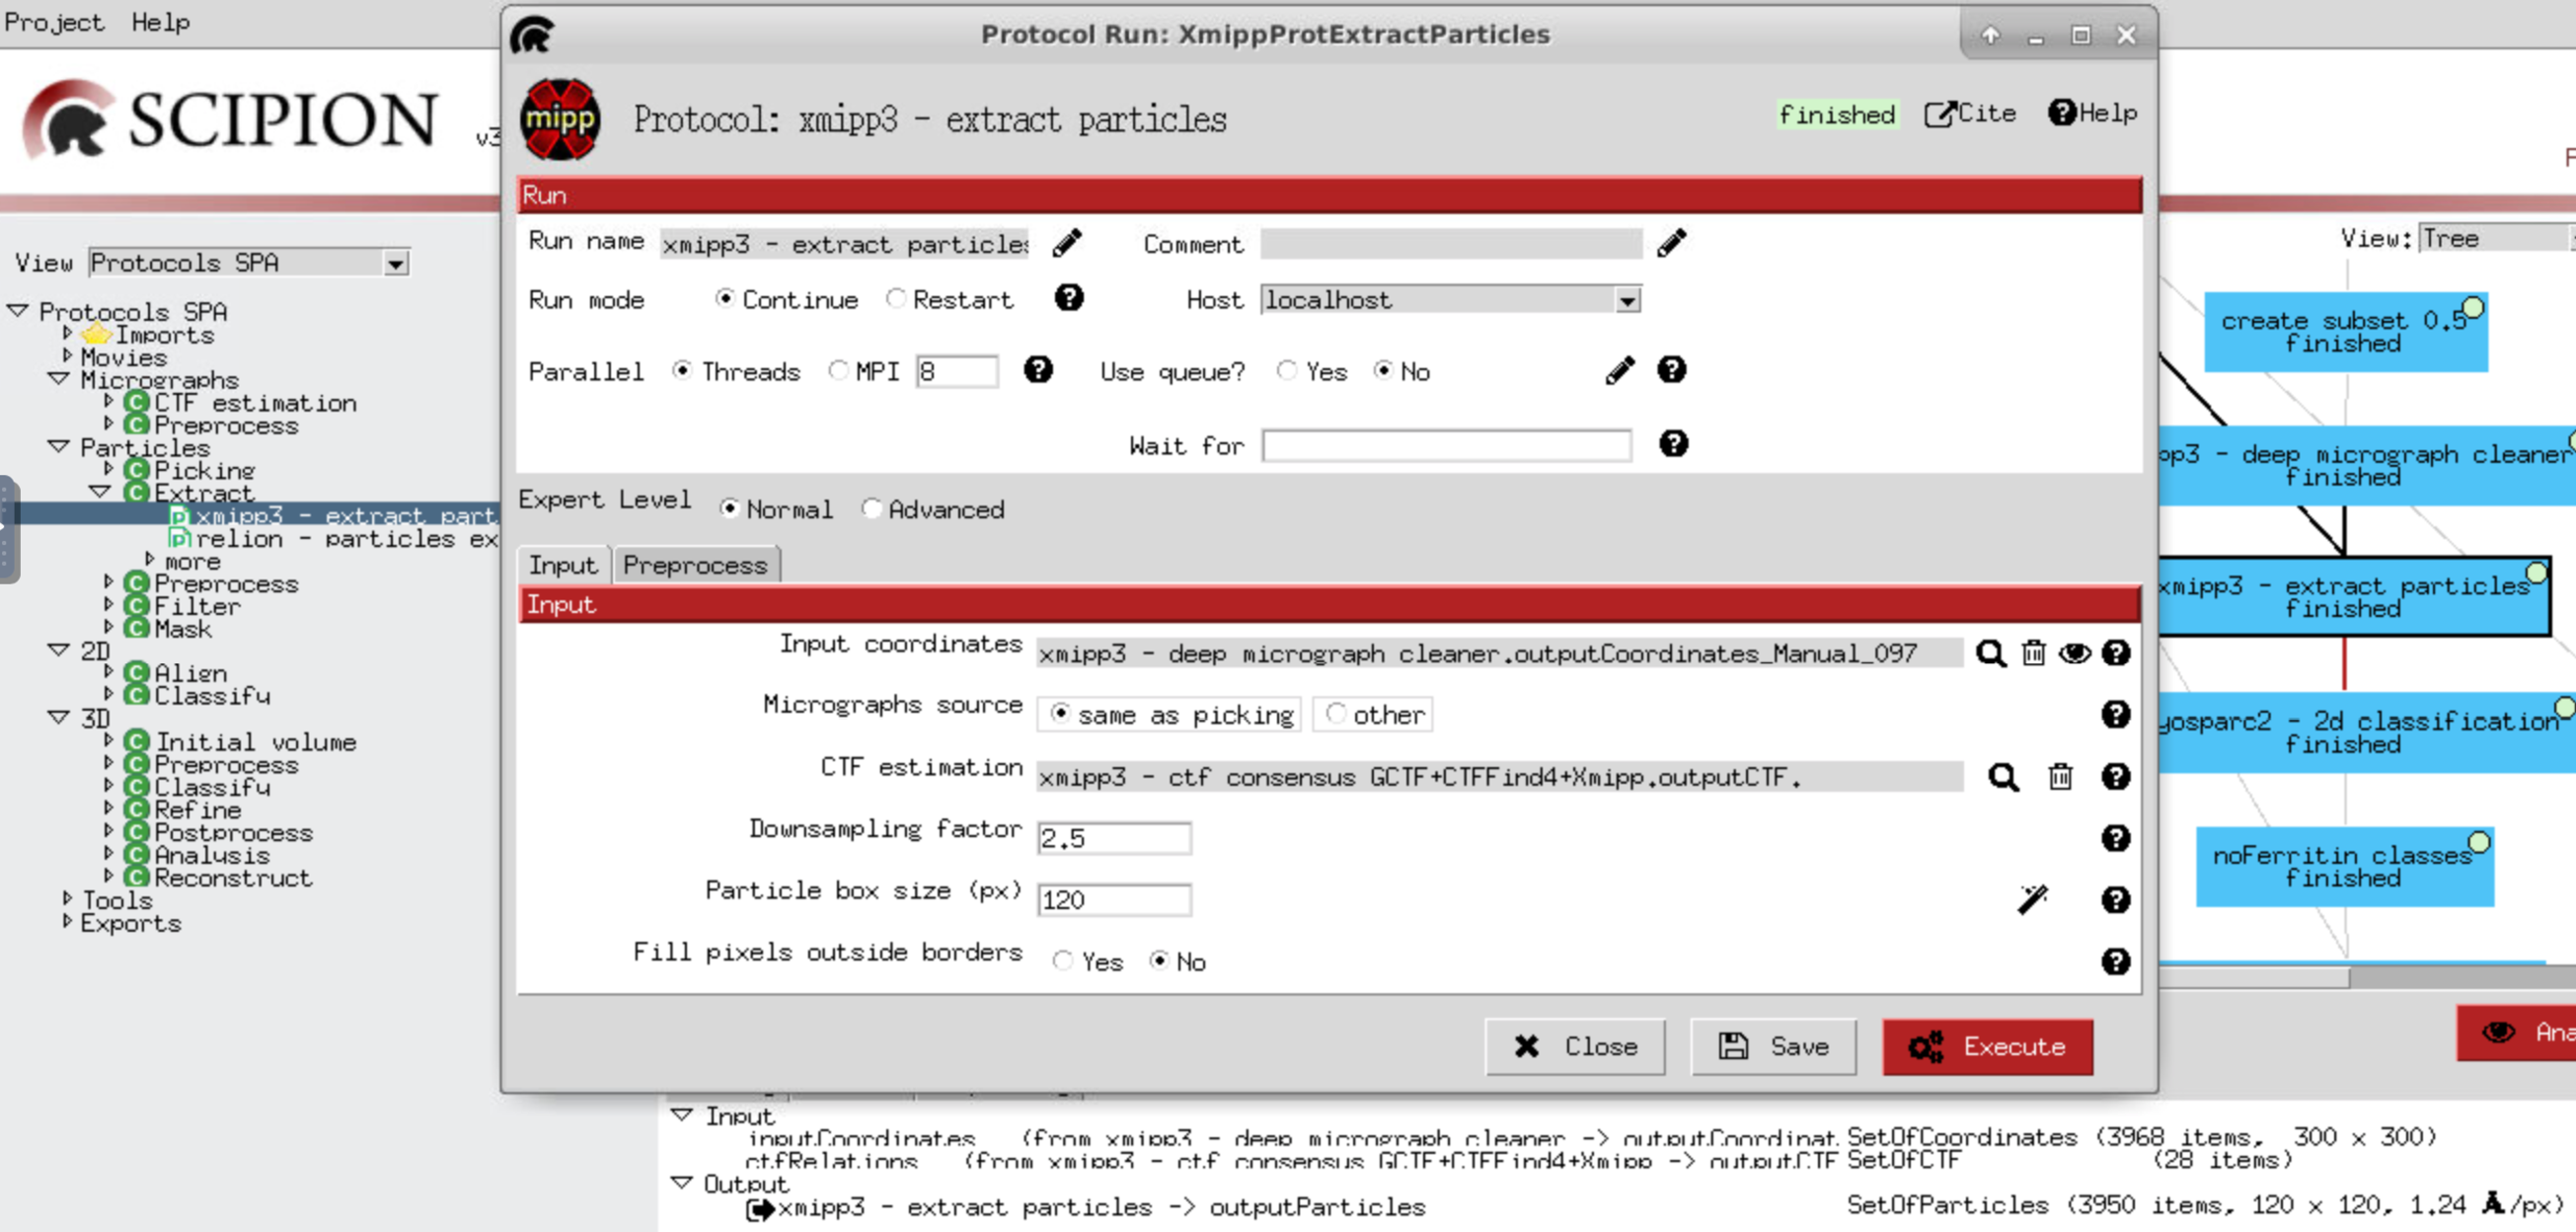
\includegraphics[width=0.95\textwidth]
  {images/6a_xmipp3_extract_particles.pdf}
  \caption{Filling in the protocol \scommand{xmipp3-extract particles}.}
  \label{fig:xmipp_extract_particles}
  \end{figure}
  
  The form tap \ttt{Preprocess} gives you additional options:
  \begin{itemize}
   \item \ttt{Dust removal}: Option \ttt{Yes} (recommended) sets pixels with unusually large values to random values from a Gaussian with zero-mean and unity-standard deviation.
   \item \ttt{Invert contrast}: Option \ttt{Yes} means that bright regions become dark and the other way around.
   \item \ttt{Phase flipping}: Option \ttt{Yes} means that the protocol corrects \ttt{CTF} phases of the particles.
   \item \ttt{Normalize}: Option \ttt{Yes} (recommended) means that the particles are normalized with zero mean and one as standard deviation for background pixels.
  \end{itemize}

  As output, the protocol generates a new set of 3,950 particles after discarding other 18 particles. The extracted particles have a smaller selected size and almost 3 times the initial sampling rate. The images of the normalized extracted particles can be seen pressing \scommand{Analyze Results}. By default, particles displayed in gallery mode can be sorted by \ttt{Zscore}. To visualize the score associated to each particle, switch the table view by pressing the top left button. If you want to remove any of the particles showing lower score values, select them, press the mouse right button and choose \ttt{Disable}. A new subset of particles can be created by clicking on \ttt{Particles} red button. However, this new subset of selected particles is considered reliable for further image processing.
